\documentclass[10pt]{scrreprt}
\usepackage[utf8]{inputenc}
\usepackage{amsfonts}
\usepackage{amsmath}
\usepackage{amssymb}
\usepackage{commath}
\usepackage[ngerman]{babel}
\usepackage{enumitem}
\usepackage{booktabs}
\usepackage{longtable}
\usepackage{relsize}
\usepackage{pgfplots}
\usepackage{csvsimple}
\usepackage{pgfplotstable}
\usepackage{siunitx}
\usepackage{fancyhdr}
\usepackage{color}
\usepackage{float}
\usepackage{listings}
\usepackage{graphicx}
\usepackage{subcaption}
\usepackage[europeanresistors]{circuitikz}

\definecolor{mygreen}{RGB}{28,172,0} % color values Red, Green, Blue
\definecolor{mylilas}{RGB}{170,55,241}


\lstset{language=Matlab,%
%basicstyle=\color{red},
breaklines=true,%
morekeywords={matlab2tikz},
keywordstyle=\color{blue},%
morekeywords=[2]{1}, keywordstyle=[2]{\color{black}},
identifierstyle=\color{black},%
stringstyle=\color{mylilas},
commentstyle=\color{mygreen},%
showstringspaces=false,%without this there will be a symbol in the places where there is a space
%numbers=left,%
%numberstyle={\tiny \color{black}},% size of the numbers
%numbersep=9pt, % this defines how far the numbers are from the text
emph=[1]{for,end,break},emphstyle=[1]\color{red}, %some words to emphasise
%emph=[2]{word1,word2}, emphstyle=[2]{style},
}

\setlength\parindent{0pt}

\setcounter{chapter}{3}
\setcounter{secnumdepth}{3}
\setcounter{figure}{12}


\pagestyle{fancy}
\fancyhf{}
\lhead{GPET Versuch 8}
\rhead{Tim Luchterhand, Paul Nykiel}
\cfoot{\thepage}

\author{Tim Luchterhand, Paul Nykiel \protect\\ tim.luchterhand@uni-ulm.de, paul.nykiel@uni-ulm.de}
\title{GPET Versuch 8 --- Karl-Ferdinand-Braun-Versuch}
\subtitle{Gruppe: Dienstag14}

\begin{document}
    \maketitle
    \section{Kennlinien von Ge- und Si-Dioden}
    \begin{figure}[H]
        \begin{subfigure}{.5\textwidth}
            \centering
            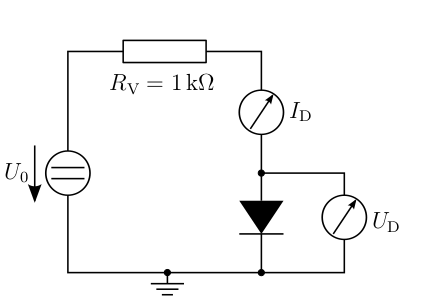
\includegraphics[width=\linewidth]{abb13a.png}
            \subcaption{}
            \label{fig:abb13a}
        \end{subfigure}
        \begin{subfigure}{.5\textwidth}
            \centering
            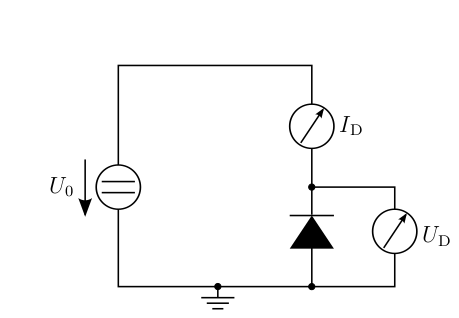
\includegraphics[width=\linewidth]{abb13b.png}
            \subcaption{}
            \label{fig:abb13b}
        \end{subfigure}
        \caption{Messaufbau für die Kennlinienbestimmung im (a) Durchlassbereich und (b) Sperrbereich.}
    \end{figure}
    Nehmen Sie zunächst die Kennlinien einer Ge- und einer Si-Diode im Durchlassbereich
    auf. Da die im Praktikum verwendeten Multimeter \textit{Agilent U1232A} im Bereich von $600\si{\mu \ampere}$
    bis $10\si{m\ampere}$ sehr ungenaue Messwerte ausgeben müssen Sie stattdessen die Schaltung aus
    Vorbereitungsaufgabe 2.2 verwenden, bei der Sie die Messschaltung aus Abbildung~\ref{fig:abb13a}
    für die Spannungsmessung angepasst haben. Verwenden Sie auf alle Fälle einen Vorwiderstand
    $R_V = 1\si{k\ohm}$, da die Dioden sonst zerstört werden können. Verwenden Sie Kanal CH1
    oder CH2 der Spannungsquelle und und achten Sie auf einen maximalen Diodenstrom
    von $20\si{m\ampere}$. Bei einem Vorwiderstand $R_V = 1\si{k\ohm}$ bedeutet dies, dass Sie maximal eine
    Spannung von $20\si{\volt}$ anlegen dürfen. Sollten Sie mit dem Aufbau unsicher sein, sprechen
    Sie Ihren Betreuer an.

    Um die Messungen zu beschleunigen, sollten Sie das automatisierte Messskript, das in
    Abschnitt 1.5 vorgestellt wurde, verwenden. Nehmen Sie pro Diode mindestens 30 Messwerte
    auf.

    Nehmen Sie anschließend die Kennlinien der beiden Diodentypen im Sperrbereich unter
    Verwendung des Messaufbaus aus Abbildung~\ref{fig:abb13b} auf. Stellen Sie das Multimeter dabei
    auf den Messbereich $\si{\mu \ampere}$. Achten Sie darauf, dass maximal $600\si{\mu \ampere}$ fließen und die
    Diodenspannung $30\si{\volt}$ nicht übersteigt. Wenn Sie die Polarität der Multimeter richtig wählen,
    erhalten Sie von vornherein das richtige Vorzeichen der Messwerte für Ihre Diodenkennlinie.

    Kombinieren Sie die Messwerte für Sperr- und Durchlassbereich und tragen Sie die Di-
    odenkennlinien unter Verwendung von MATLAB oder EXCEL in linearer Darstellung in
    ein gemeinsames Diagramm ein. Zeichnen Sie außerdem ein weiteres Diagramm, das nur
    den Durchlassbereich zeigt und bestimmen Sie die Schwellenspannung $U_S$ bei der $1\si{m\ampere}$
    Strom fließt. Welche Unterschiede zwischen Ge- und Si-Dioden fallen Ihnen auf?
    Tragen Sie nun jeweils die Kennlinien für den Durchlassbereich in halblogarithmischer
    Darstellung auf. Bestimmen Sie nun den Emissionskoeffizienten n für die beiden Dioden-
    typen. Betrachten Sie hierfür zunächst die halblogarithmische Kennlinie und begründen
    Sie, warum Sie nur Messpunkte mit geringen Strömen ($I_D < 100\si{\mu\ampere}$) für die Bestimmung
    des Serienwiderstandes wählen dürfen. Welchen weiteren Effekt könnten Sie mit einem
    Messpunkt bei höheren Strömen berechnen?

    \paragraph{Protokoll}
    $ $
    \begin{figure}[H]
        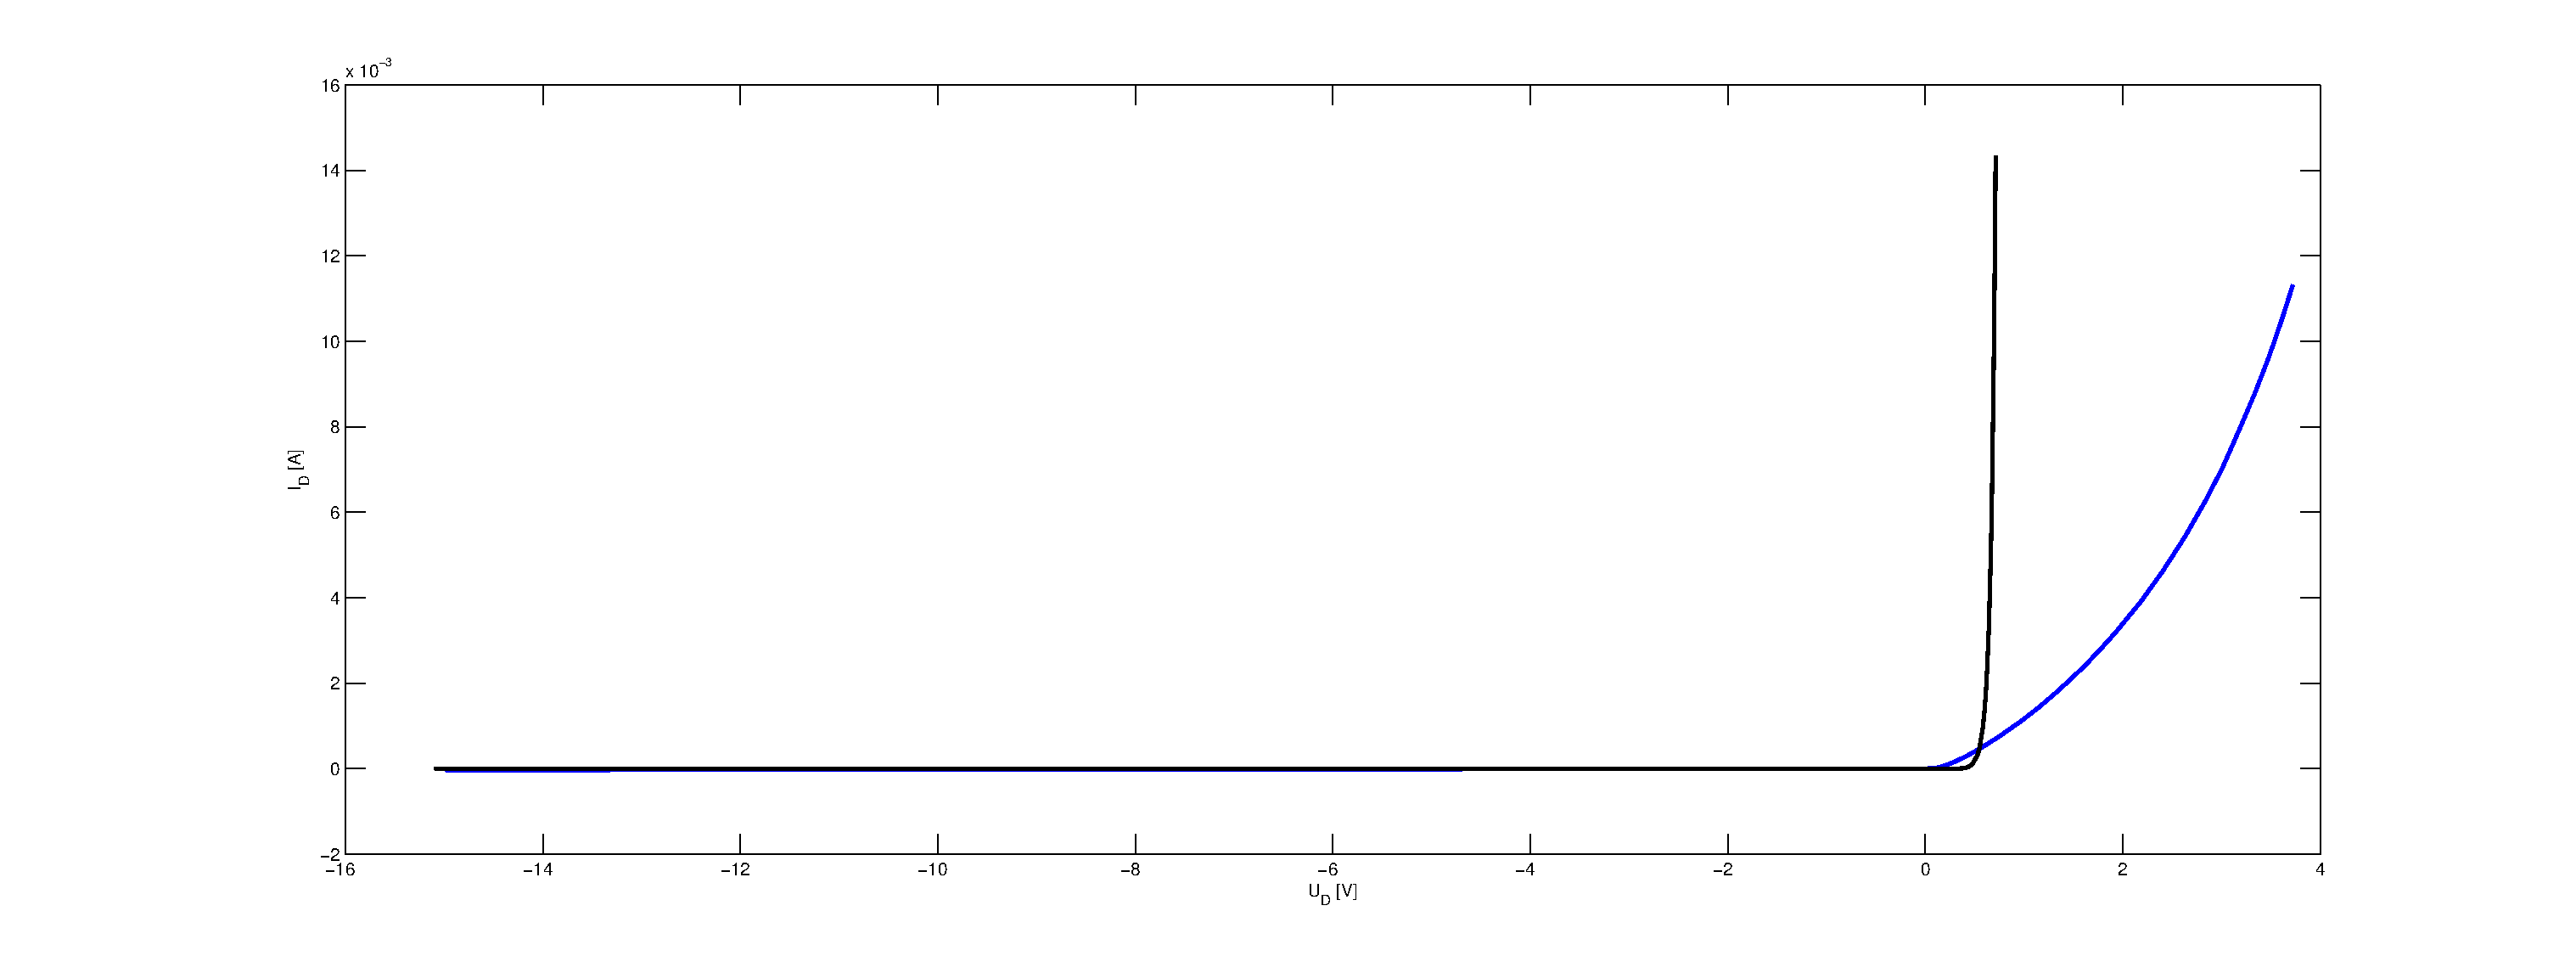
\includegraphics[width=\textwidth]{GeSiGes}
        \caption{Vollständige Diodenkennlinie (Si-Diode in Schwarz, Ge-Diode in Blau)}
    \end{figure}

    Auffällig ist, dass der Diodenstrom bei der Germanium-Diode deutlich langsamer
    ansteigt, als bei der Silizuim-Diode.

    \begin{figure}[H]
        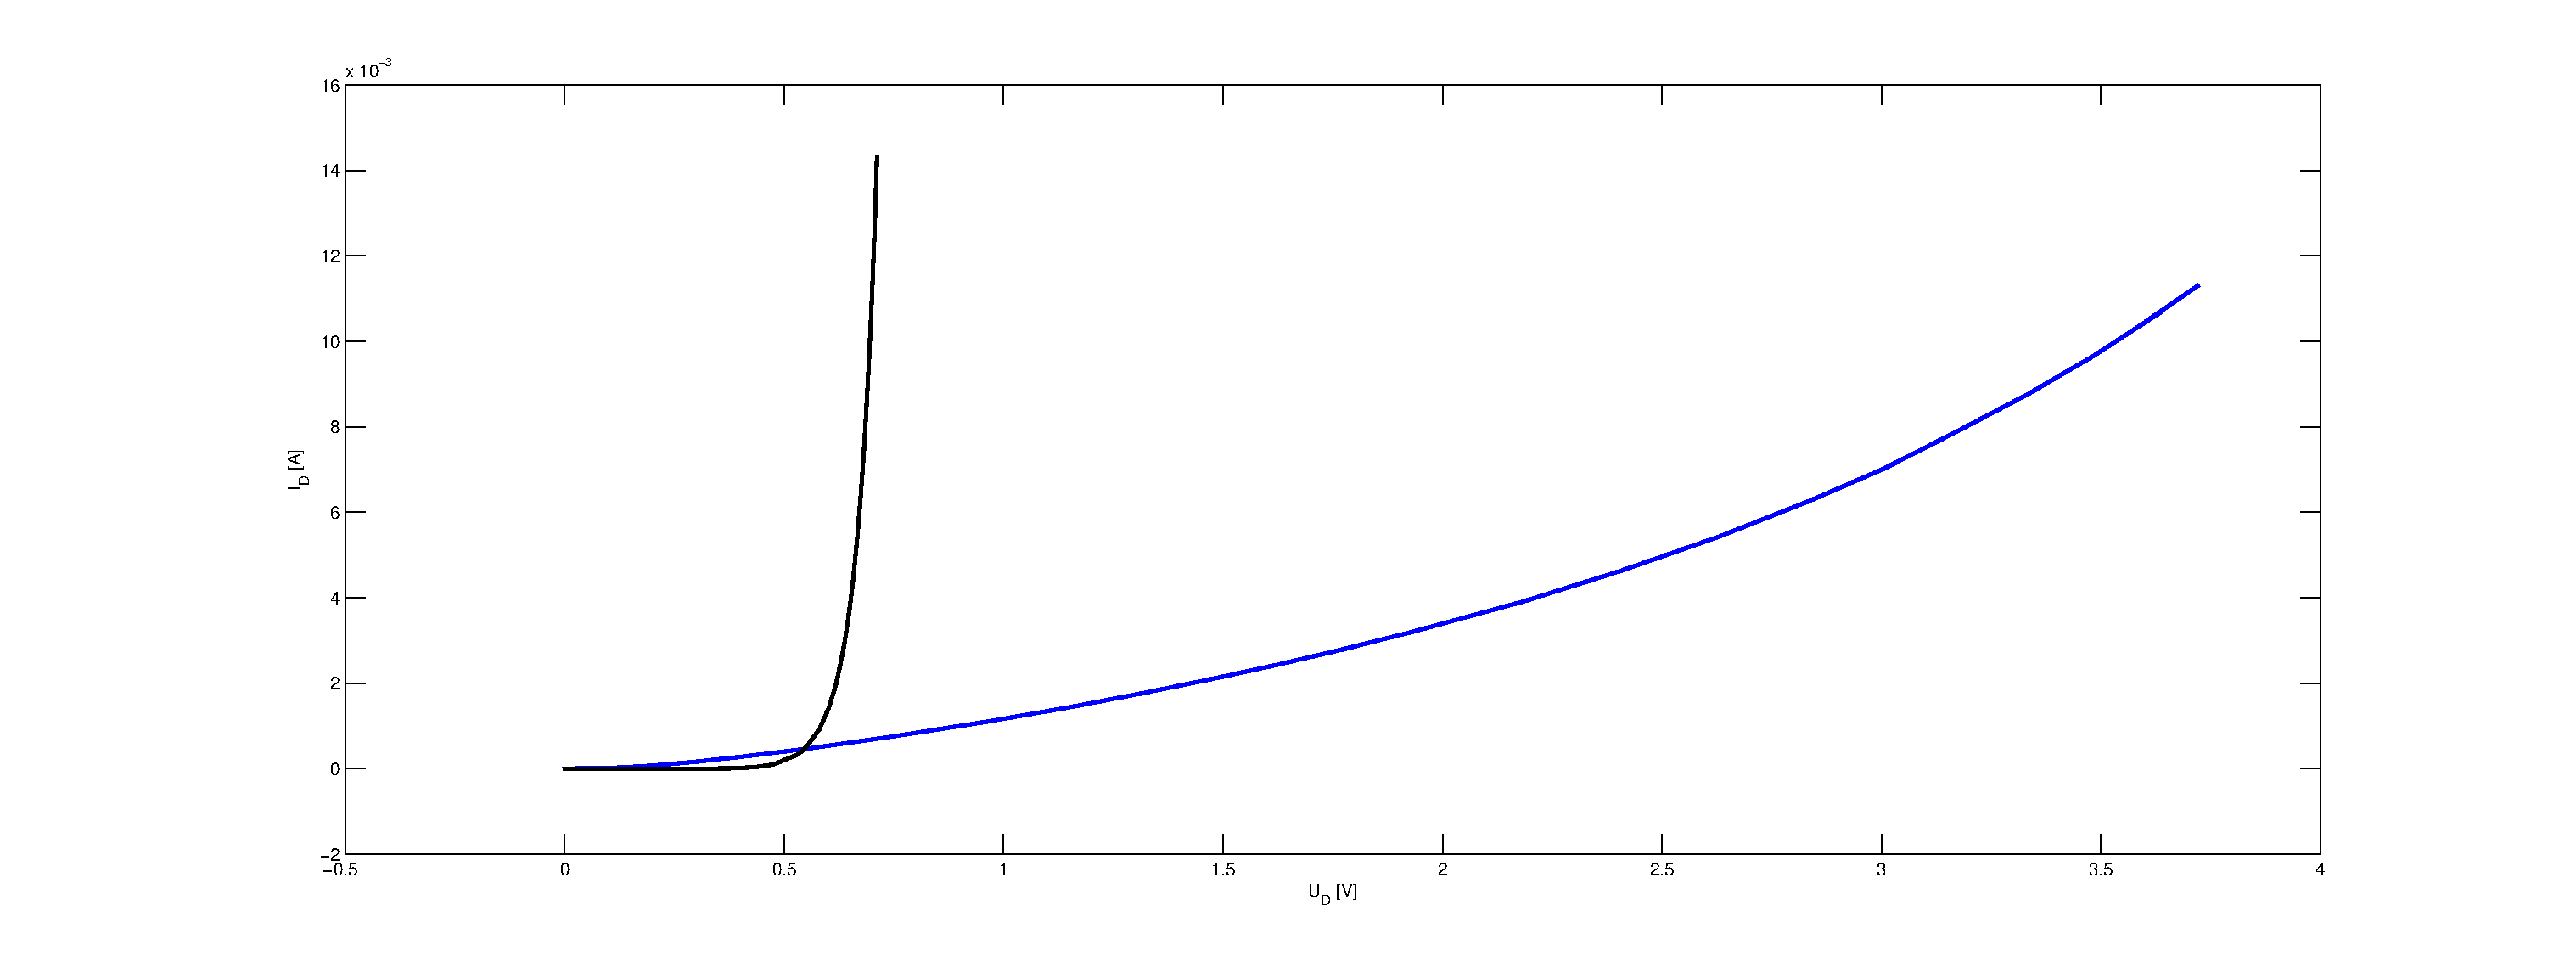
\includegraphics[width=\textwidth]{GeSiDurch}
        \caption{Diodenkennlinie im Durchlassbereich (Si-Diode in Schwarz, Ge-Diode in Blau)}
        \end{figure}
        \begin{figure}[H]
        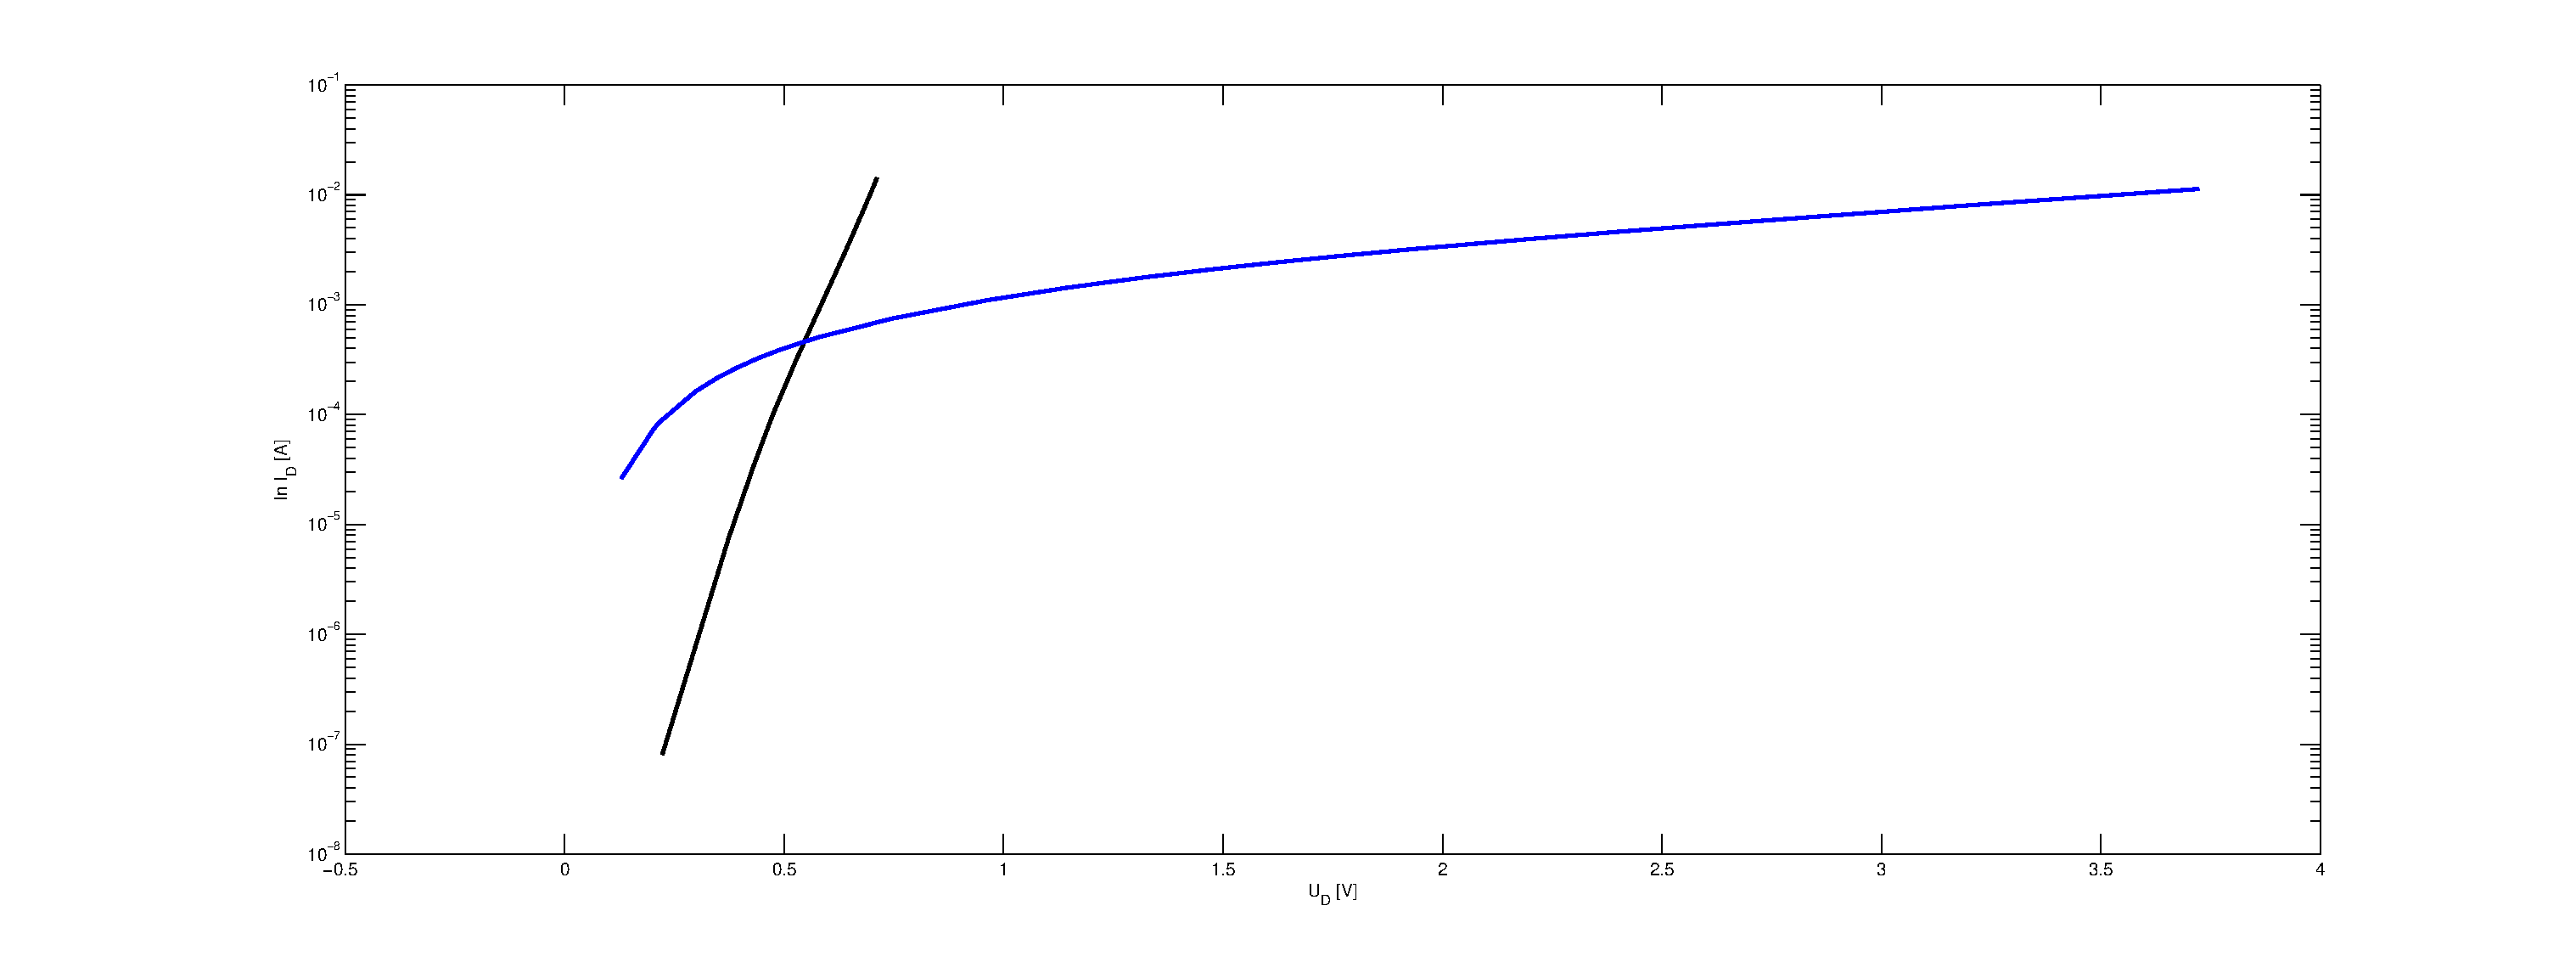
\includegraphics[width=\textwidth]{GeSiDurchLog}
        \caption{Logarithmische Diodenkennlinie in Durchlassrichtung (Si-Diode in Schwarz, Ge-Diode in Blau)}
        \label{fig:logzeug}
    \end{figure}


    Der Emissionskoeffizient für die Germanium-Diode lässt sich folgendermaßen berechen:
    \begin{eqnarray*}
        U_1 &=& 0.15\si{\volt}\\
        U_2 &=& 0.25\si{\volt}\\
        I_1 &=& \SI{1.15e-5}{\ampere}\\
        I_2 &=& \SI{1.8e-5}{\ampere}\\
        n &=& \frac{U_2 - U_1}{U_T\ln\left(\frac{I_2}{I_1}\right)} = 8.58
    \end{eqnarray*}

    Für die Silizumdiode ergibt sich folgendes:
    \begin{eqnarray*}
        U_1 &=& 0.2\si{\volt}\\
        U_2 &=& 0.5\si{\volt}\\
        I_1 &=& \SI{1.7e-8}{\ampere}\\
        I_2 &=& \SI{1.5e-5}{\ampere}\\
        n &=& 1.7
    \end{eqnarray*}

    Bei der Bestimmung von n wurden nur Messpunkte betrachtet, bei denen der Diodendtrom
    kleiner als $10^{-4}\si{\ampere}$ ist, betrachtet. Dies ist wichtig, da bei
    höheren Strömen der Bahnwiderstand der Diode ins Gewicht fällt und die Steigung
    der Kennlinie verändert (wie auch in~\ref{fig:logzeug} zu sehen).

    \section{Kennlinie einer Z-Diode}
    Nehmen Sie nun die Kennlinie der Zener-Diode auf und tragen Sie Sie in linearer Darstellung
    in ein Diagramm ein. Für den Durchlassbereich verwenden Sie die modifizierte
    Schaltung aus Aufgabe 2.2. Überlegen Sie wie die Messschaltung für die Zener-Diode für
    den Sperrbereich aussehen muss und begründen Sie Ihre Entscheidung. Im Sperrbereich
    dürfen maximal $20\si{m\ampere}$ fließen. Sollten Sie bezüglich des Messaufbaus unsicher sein, fragen
    Sie Ihren Betreuer, da die Dioden ansonsten zerstört werden können.

    \paragraph{Protokoll}
    Die Messschaltung muss im Sperrbereich identisch der Schaltung im Durchlassbereich
    sein, da die Diode auch für Spannungen kleiner der Durchbruchspannung leitet.
    Ohne den Widerstand würde die Diode sonst kurzgeschlossen. Im Durchlassbereich
    verhält sich die Z-Diode wie eine normale Diode.

    \begin{figure}[H]
        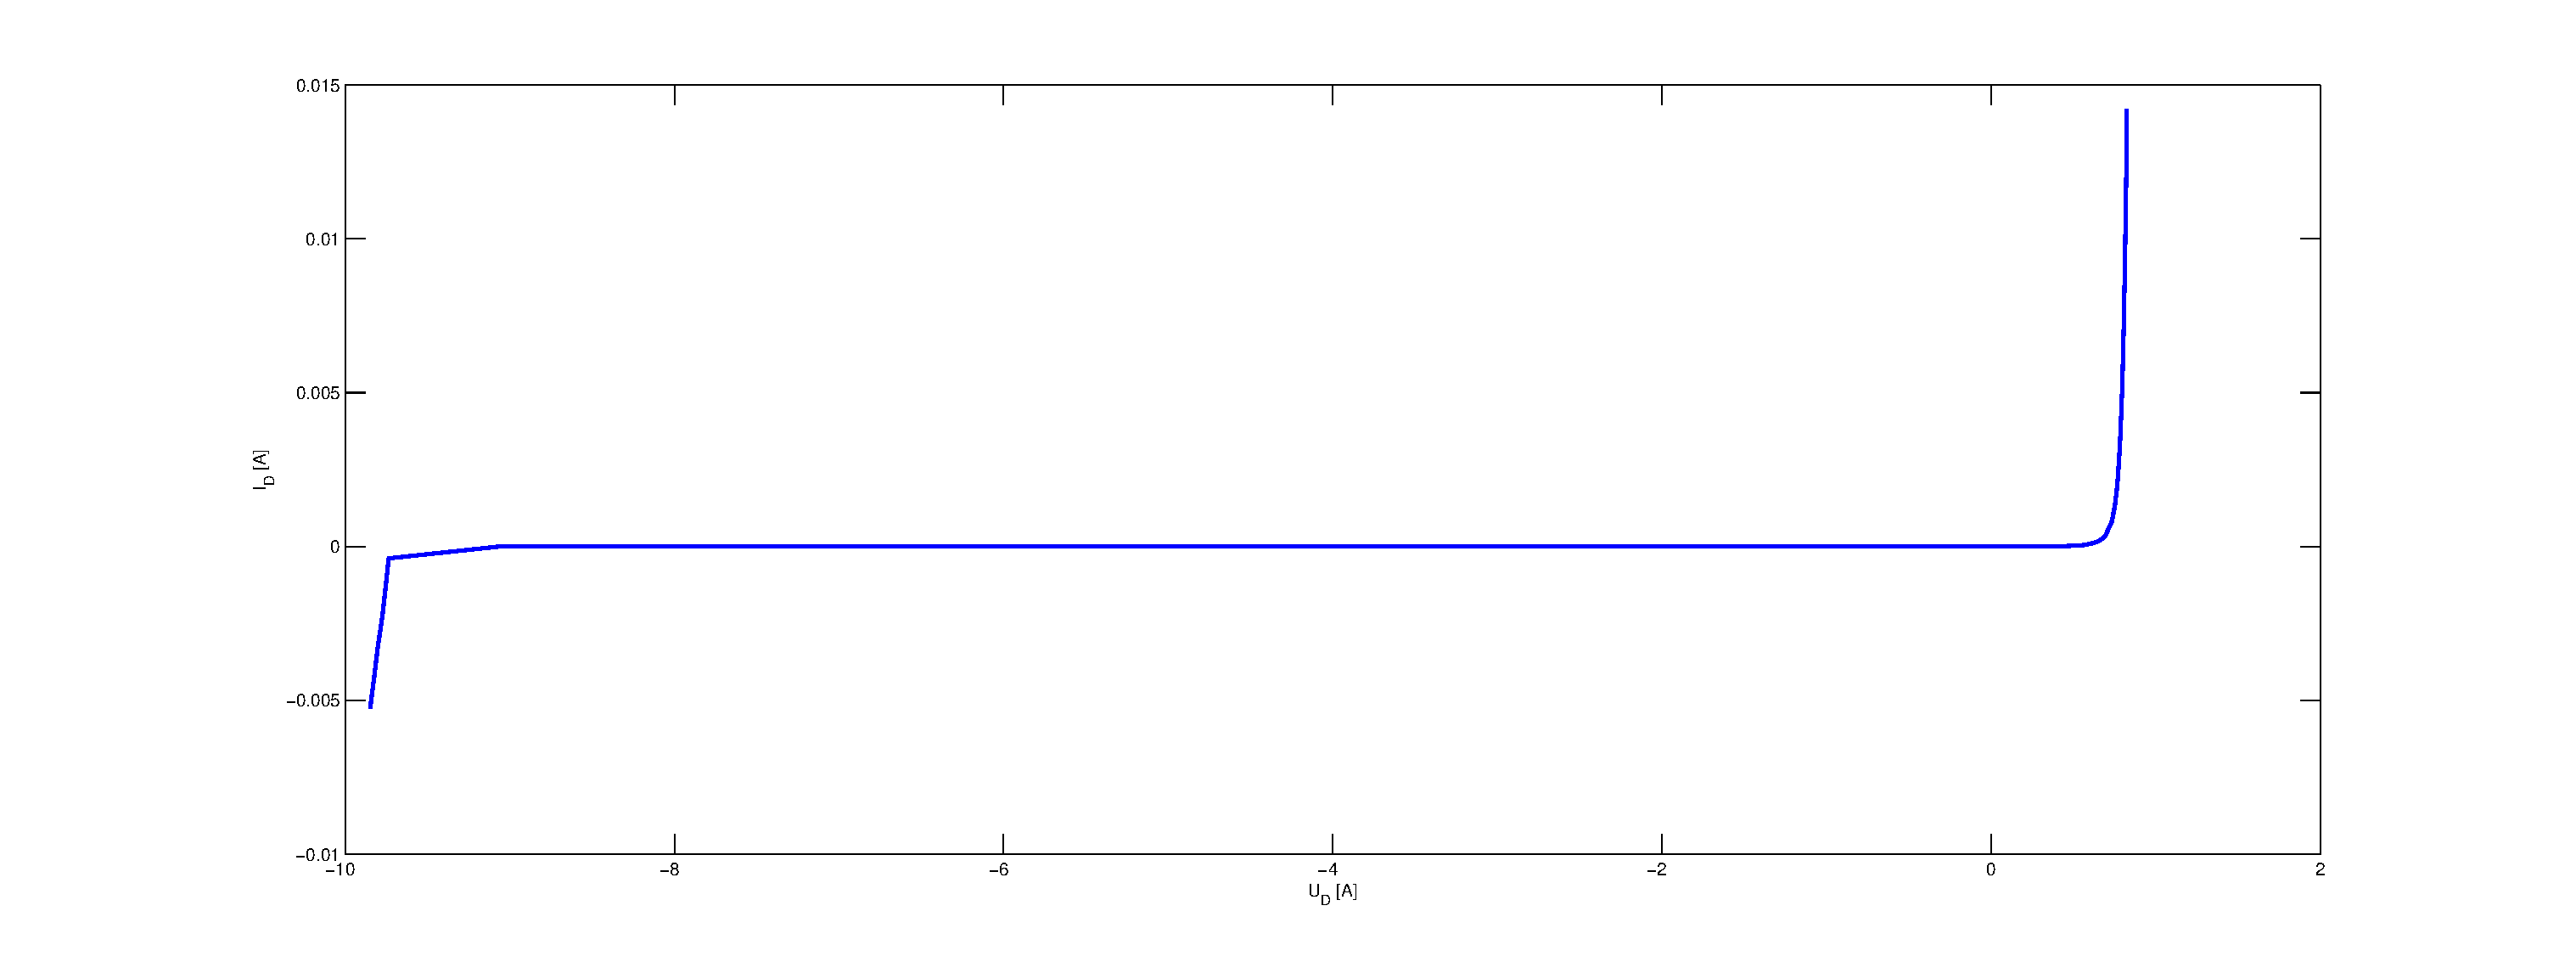
\includegraphics[width=\textwidth]{ZGes}
        \caption{Diodenkennlinie der Zener-Diode}
        \label{fig:ZDiode}
    \end{figure}

    Bemerkung: Wie aus Diagramm~\ref{fig:ZDiode} hervorgeht, besitzt die Z-Diode
    eine Durchbruchspannung von ca.~$-9\si{\volt}$.

    \section{Begrenzerschaltungen}
    Bauen Sie die Begrenzerschaltung aus Abbildung~\ref{fig:abb14} mit Silizium-Dioden auf und achten
    Sie darauf, den korrekten Vorwiderstand zu verwenden. Varriieren Sie nun die Eingangsspannung
    $U_{in}$ zwischen $-15\si{\volt}$ bis $15\si{\volt}$ in Schritten von $1\si{\volt}$ und nehmen Sie mit Hilfe des
    Messkriptes sowohl die Eingangsspannung $U_{in}$ als auch die Ausgangsspannung $U_{out}$ mit
    Hilfe zweier Multimeter auf.
    \begin{figure}[H]
        \centering
        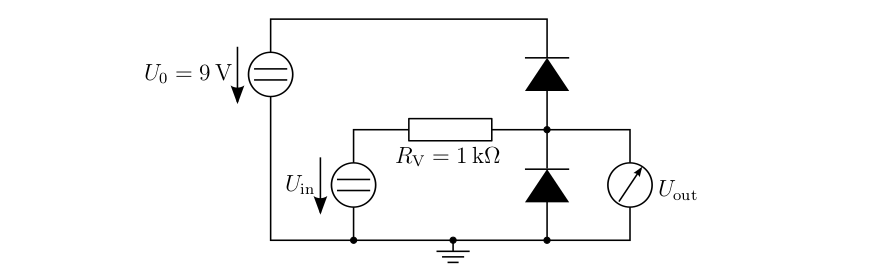
\includegraphics[width=\textwidth]{abb14.png}
        \caption{Begrenzerschaltung mit zwei Dioden.}
        \label{fig:abb14}
    \end{figure}
    In Aufgabe 2.3 haben Sie eine vereinfachte Form der Schaltung entworfen. Bauen Sie
    diese auf und verifizieren Sie die Funktionalität indem Sie auch hier die
    Ausgangscharakteristik messen. Stellen für beide Schaltungen die Ausgangsspannung als
    Funktion der Eingangsspannung $U_{out} (U_{in})$ in einem gemeinsamen Diagramm dar.
    Erklären Sie, wozu eine solche Schaltung eingesetzt werden könnte.

    \paragraph{Protokoll}
    $ $
    \begin{figure}[H]
        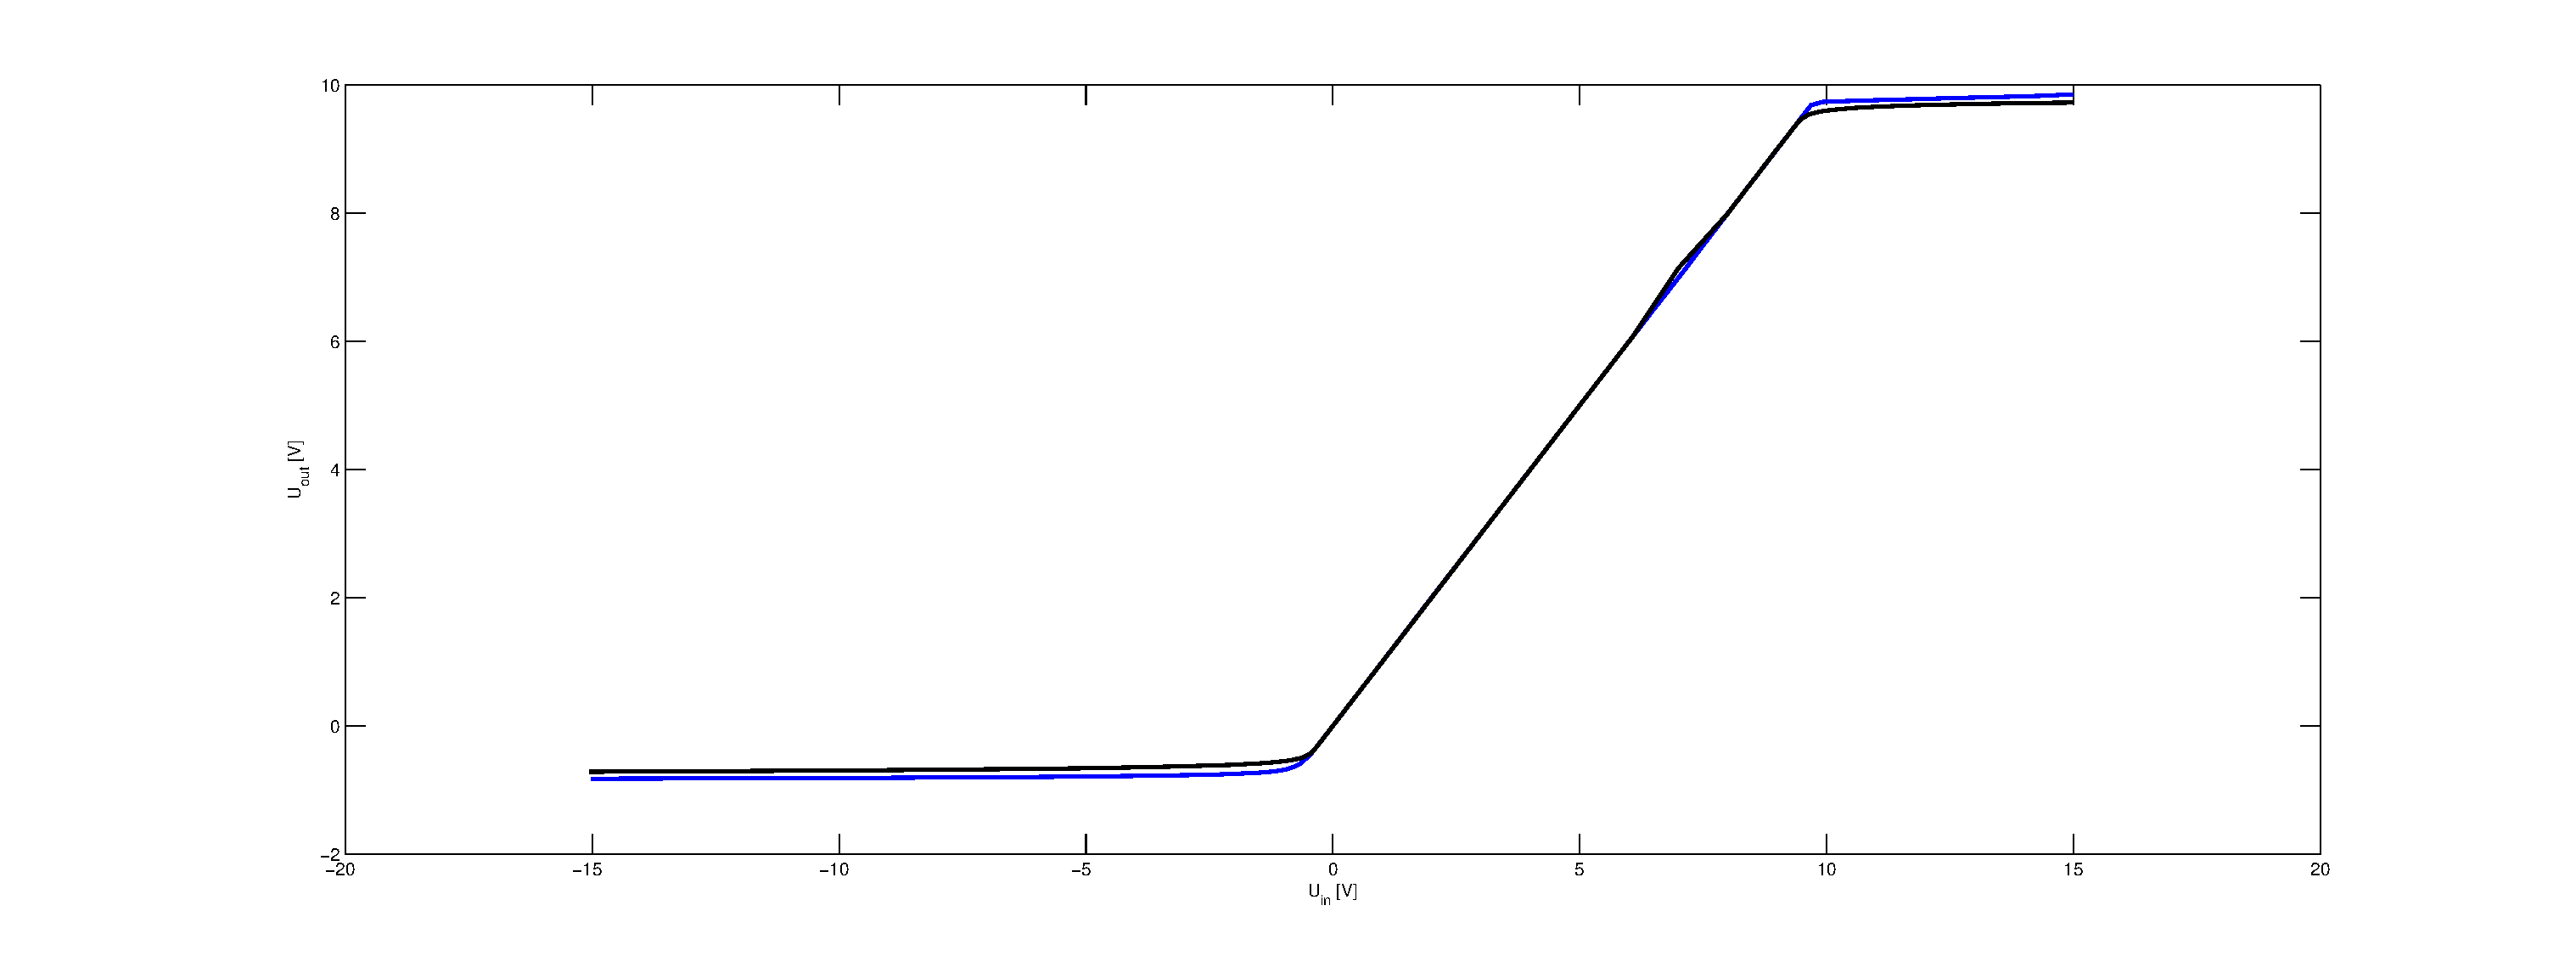
\includegraphics[width=\textwidth]{BegrGes}
        \caption{Begrenzerschaltung (vereinfacht in blau, kompliziert in schwarz)}
    \end{figure}

    Die Begrenzerschaltung begrenzt Spannungen nach oben auf einen vorher
    festgelegten Wert. Außerdem werden negative Spannungen unterdrückt. Dies ist
    z.B.~dann sinnvoll, wenn man empfindliche Geräte, die kein zu hohen oder negative
    Spannungen vertragen, absichern will.

    \section{Graetz-Gleichrichter}
    \begin{figure}[H]
        \centering
        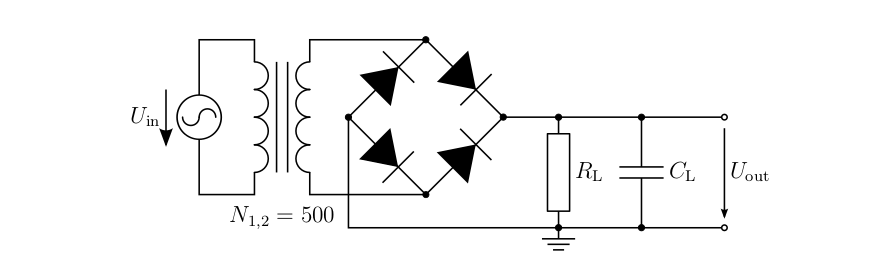
\includegraphics[width=\textwidth]{abb15.png}
        \caption{Messaufbau des Graetz-Gleichrichters mit Transformator.}
        \label{fig:abb15}
    \end{figure}
    Bauen Sie den Brückengleichrichter nach Abbildung~\ref{fig:abb15} mit Silizium-Dioden auf.
    Generieren Sie das Eingangssignal $U_{in}$ mit Hilfe des Frequenzgenerators im Oszilloskop, stellen
    Sie dabei ein Sinussignal mit einer Amplitude von $U_{pp} = 5\si{\volt}$ und einer Frequenz von
    $f_{in} = 1\si{k\hertz}$ ein.

    Messen Sie für folgende Kombinationen aus $R_L$ und $C_L$ die zeitlichen Ausgangssignale mit
    dem Oszilloskop und stellen Sie es zusammen mit dem Eingangssignal dar. Sie können
    hierfür die MATLAB -GUI oder die Save-Funktion des Oszilloskopes nutzen. Bestimmen
    Sie außerdem für jedes Ausgangssignal die Amplitude $U_{out,pp}$ der Restwelligkeit und den
    RMS-Wert $U_{out,RMS}$ des Ausgangssignals.

    \begin{enumerate}
        \item $R_L  = 10\si{k \ohm}$, $C_L$ entfernt
        \item $R_L  = 10\si{k \ohm}$, $C_L = 100\si{n\farad}$ (Die $100\si{n\farad}$ Kondensatoren sind
            häufig aus einem früheren Versuch mit schwarzem Klebeband abgeklebt)
        \item $R_L  = 10\si{k \ohm}, C_L = 2.2\si{\mu\farad}$
        \item $R_L  = 1\si{k \ohm}, C_L = 2.2\si{\mu \farad}$
    \end{enumerate}
    Erklären Sie die Messergebnisse. Wieso wird der Transformator für diesen Messaufbau
    benötigt?

    \paragraph{Protokoll}
    $ $

    \begin{figure}[H]
        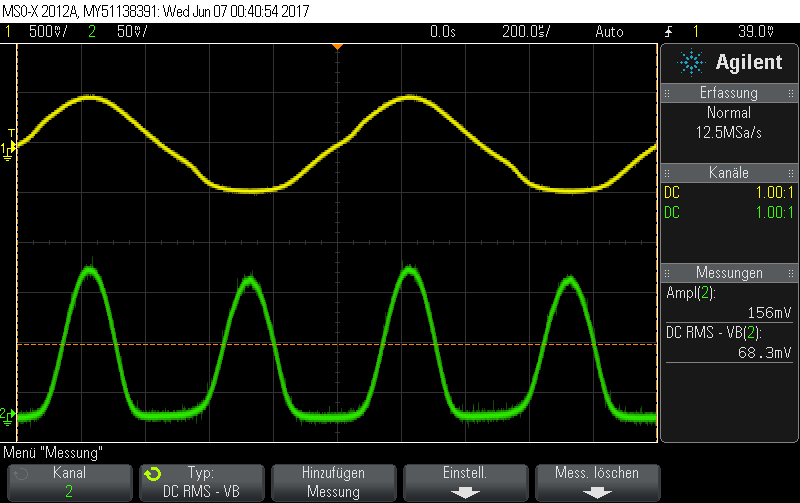
\includegraphics[width=\textwidth]{scope_4.png}
        \caption{$R_L  = 10\si{k \ohm}$, $C_L$ entfernt}
    \end{figure}

    \begin{eqnarray*}
        \hat{U} &=& 156\si{m\volt}\\
        U_{RMS} &=& 68.3\si{m\volt}\\
        \Rightarrow \omega &=& \frac{\hat{U}}{2.5\si{\volt}} = 0.0624
    \end{eqnarray*}

    Ein idealer Gleichrichter ohne Glättung würde den Betrag des Eingangssignals
    ausgeben. Da aber die verwendeten Dioden erst ab einer gewissen Schwellspannung
    durchschalten, gehen Spannungnen, die betragsmäßig kleiner sind als ca.
    $0.7\si{\volt}$, verloren. Da hier zusätzlich kein Kondensator verwendet wurde,
    gibt es auch keine Glättung und das Ausgangssignal ist eine oszillierende
    positive Spannung.

    \begin{figure}[H]
        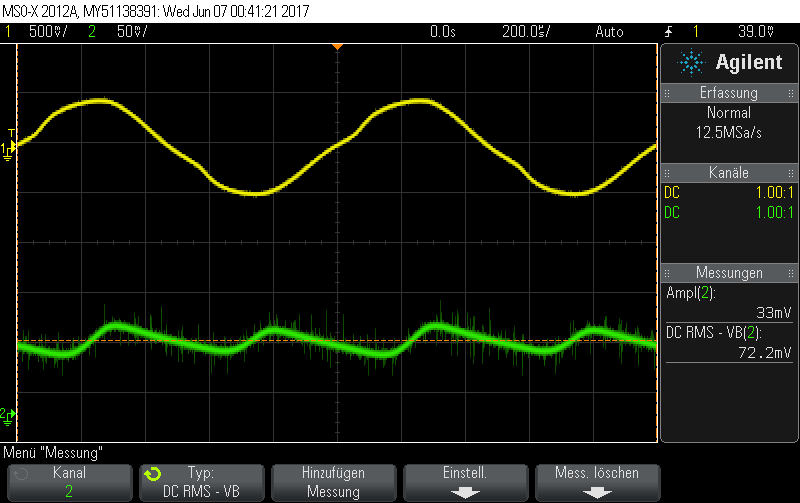
\includegraphics[width=\textwidth]{scope_5.png}
        \caption{$R_L  = 10\si{k \ohm}$, $C_L = 100\si{n\farad}$}
    \end{figure}

    \begin{eqnarray*}
        \hat{U} &=& 33\si{m\volt}\\
        U_{RMS} &=& 72.2\si{m\volt}\\
        \Rightarrow \omega &=& \frac{\hat{U}}{2.5\si{\volt}} = 0.0132
    \end{eqnarray*}

    Durch einen relativ kleinen Kondensator wird das Ausgangssignal leicht geglättet.

    \begin{figure}[H]
        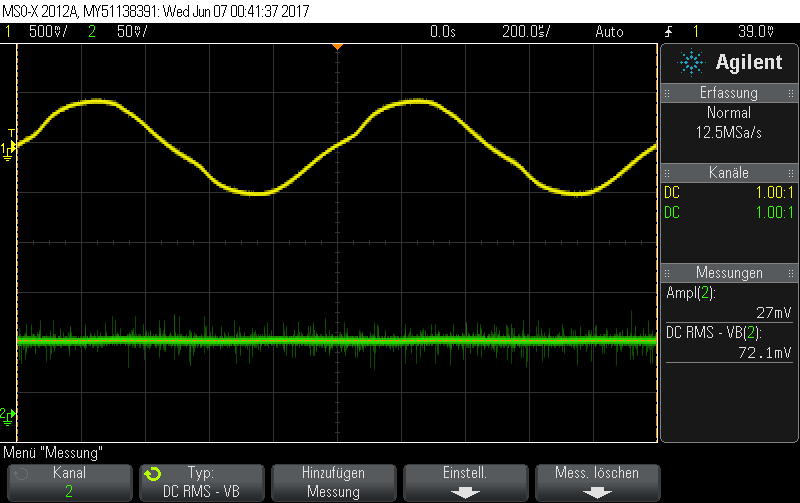
\includegraphics[width=\textwidth]{scope_6.png}
        \caption{$R_L  = 10\si{k \ohm}, C_L = 2.2\si{mu\farad}$}
        \label{fig:FuckAll}
    \end{figure}

    \begin{eqnarray*}
        \hat{U} &=& 27\si{m\volt}\\
        U_{RMS} &=& 72.1\si{m\volt}\\
        \Rightarrow \omega &=& \frac{\hat{U}}{2.5\si{\volt}} = 0.0108
    \end{eqnarray*}

    Bei einem Kondensator mit $C_L = 2.2\si{\mu\farad}$ ist die Glättung so stark,
    dass nur noch ein fast konstantes Ausgangssignal gemessen wird.

    \begin{figure}[H]
        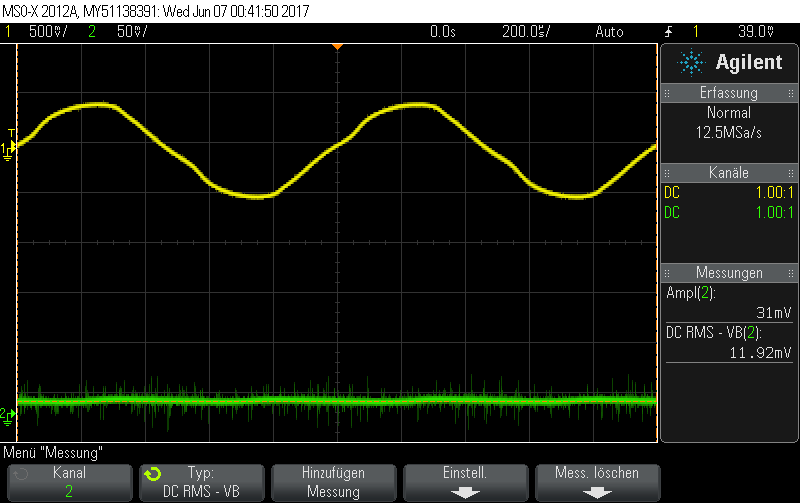
\includegraphics[width=\textwidth]{scope_7.png}
        \caption{$R_L  = 1\si{k \ohm}, C_L = 2.2\si{\mu \farad}$}
    \end{figure}

    \begin{eqnarray*}
        \hat{U} &=& 31\si{m\volt}\\
        U_{RMS} &=& 11.92\si{m\volt}\\
        \Rightarrow \omega &=& \frac{\hat{U}}{2.5\si{\volt}} = 0.0124
    \end{eqnarray*}

    Im Vergleich zu~\ref{fig:FuckAll} ist hier die Spannung des Ausgangssignals
    kleiner, da ein kleinerer Widerstand verwendet wurde. Dadurch ist aber auch
    die Amplitude und Restwelligkeit des Ausganssignals höher.

    %TODO Restwelligkeit, RMS, Amplitude, Wieso Transformator

    \section{Leuchtdioden}
    Messen Sie die Kennlinie einer LED im Durchlassbereich unter Verwendung der
    modifizierten Schaltung aus Aufgabe 2.2 mit einem maximalen Strom von $20\si{m\ampere}$ und plotten
    Sie die Kennlinie in linearer Darstellung.
    Nehmen Sie nun an, Sie möchten zwei dieser LEDs mit einem Strom von $10\si{m\ampere}$ an
    einer $5\si{\volt}$ Spannungsquelle betreiben. Schalten Sie die LEDs hierfür parallel oder seriell?
    Begründen Sie Ihre Entscheidung, berechnen Sie einen passenden Vorwiderstand für die
    LEDs und zeichnen Sie die fertige Schaltung auf.

    \subsection{Protokoll}
    $ $
    \begin{figure}[H]
        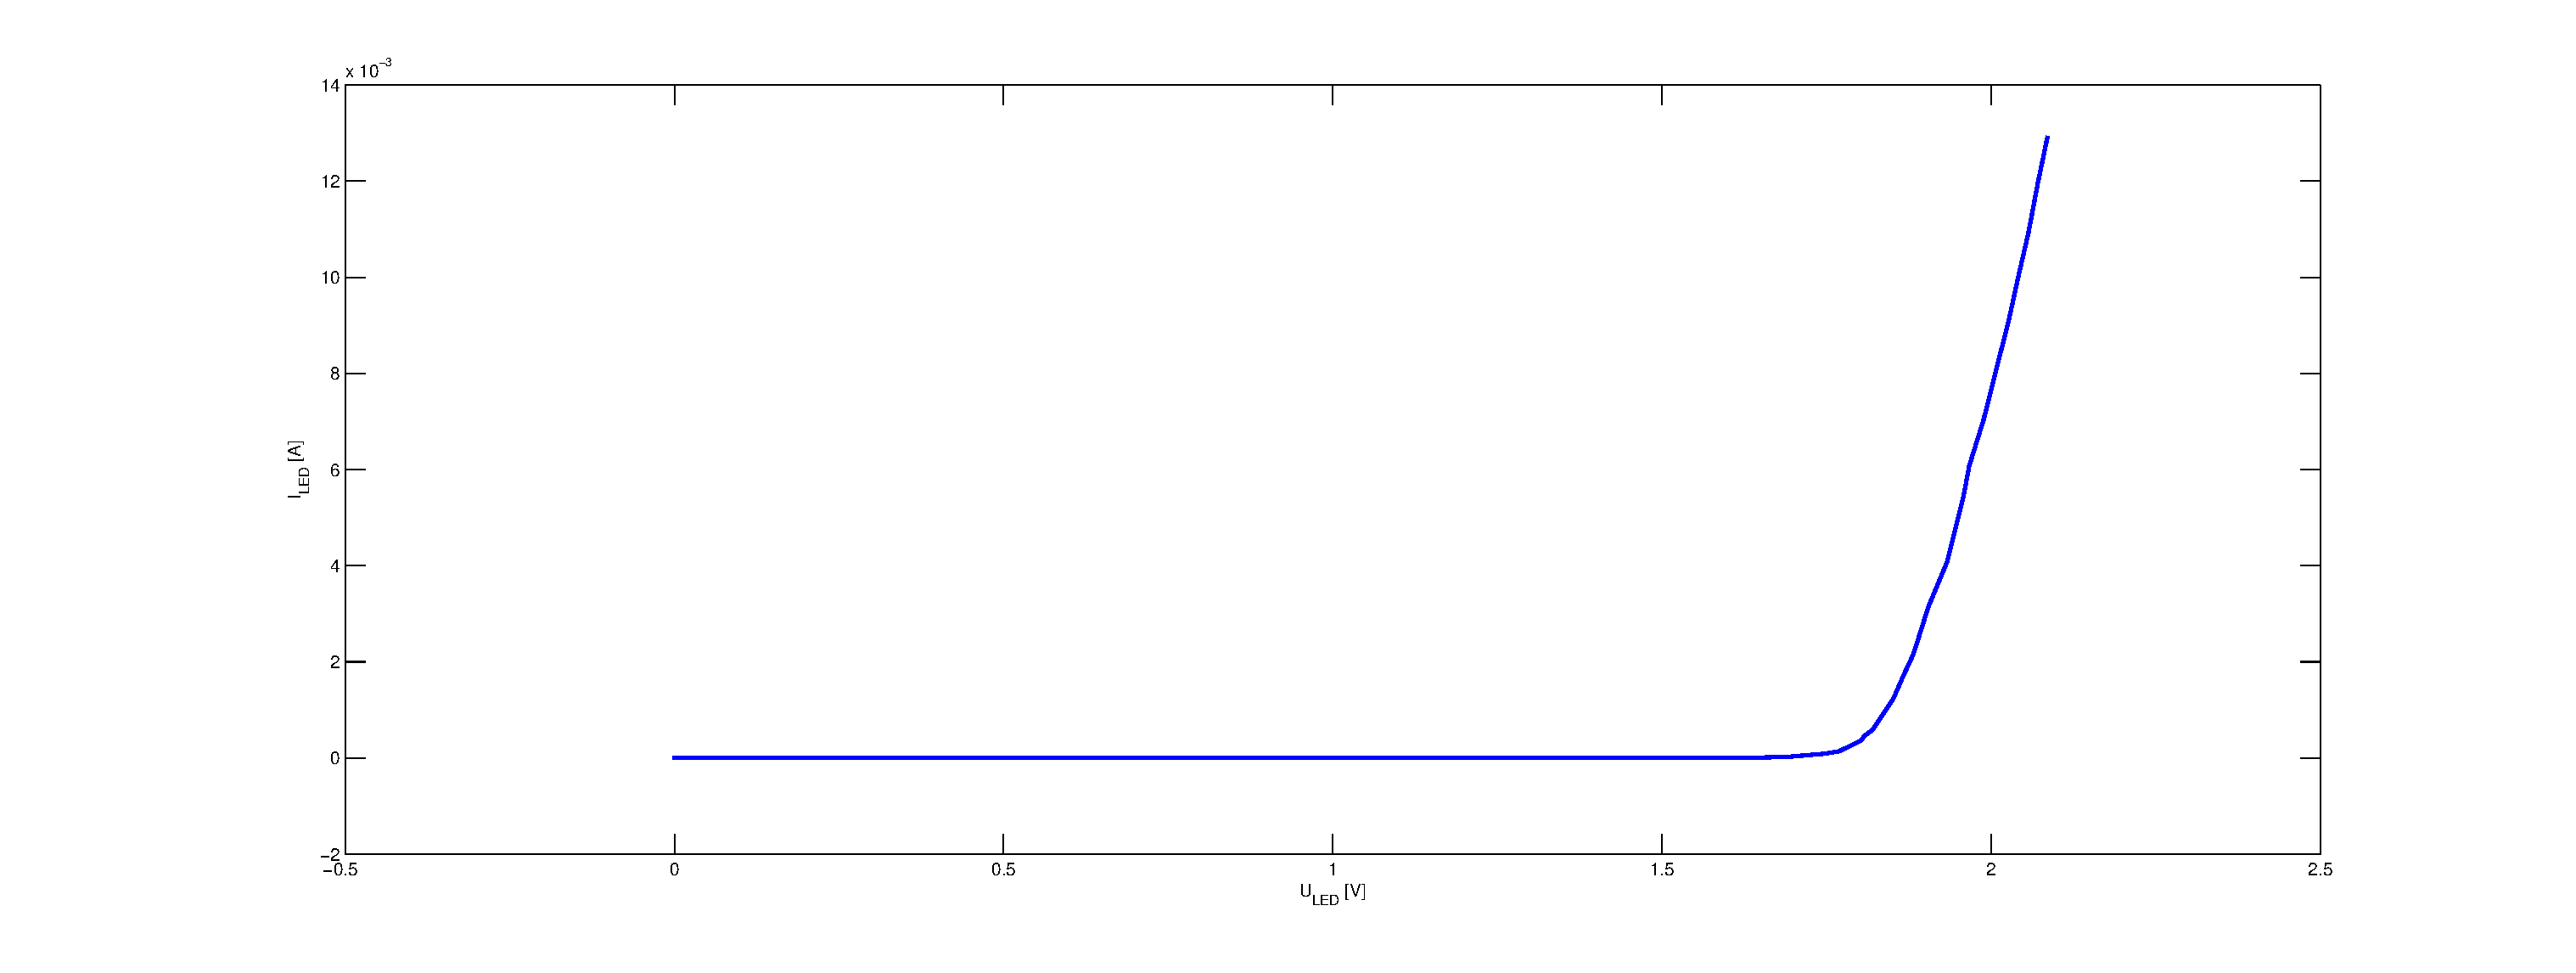
\includegraphics[width=\textwidth]{LED}
        \caption{Kennlinie der LED}
        \label{fig:led}
    \end{figure}

    Wie aus Grafik~\ref{fig:led} hervorgeht müssten an der Diode $2\si{\volt}$
    anliegen, damit ein Strom von $10\si{m\ampere}$ fließt. In einer Reihenschaltung
    von zwei Dioden müsste am Vorwiderstand 1V abfallen. Bei einem Dieodenstrom
    $I_D = I_{ges} = 10\si{m\ampere}$ ist dieser also $R_{vor} = 100\si{\ohm}$.
    Eine Reihenschaltung ist deshalb sinnvoll, da sich beide Dioden nicht perfekt
    gleich verhalten. Wenn z.B. eine der beiden Dioden bei einer niedrigeren
    Schwellspannung durchschaltet, würde der gesamte Strom nur über diese Diode
    fließen.
    \vspace{0.5cm}
    \begin{figure}[H]
        \centering
        \begin{circuitikz}
            \draw (-3, 0) to[short] (0,0);
            \draw (0,0) to[R=$R_{vor} \text{=} 100\si{\ohm}$] (0, -2);
            \draw (0,-2) to[empty led] (0,-3);
            \draw (0,-3) to[empty led] (0,-4);
            \draw (-3, -4) to[battery1, l=$5\si{\volt}$] (-3, 0);
            \draw (-3, -4) to[short] (0, -4);
        \end{circuitikz}
        \caption{Schaltung}
    \end{figure}

\end{document}
